\documentclass[11pt, oneside]{article}   	% use "amsart" instead of "article" for AMSLaTeX format


\usepackage[letterpaper, top=10mm]{geometry}
             		% See geometry.pdf to learn the layout options. There are lots.
              		% ... or a4paper or a5paper or ... 
%\geometry{landscape}                		% Activate for rotated page geometry
%\usepackage[parfill]{parskip}    		% Activate to begin paragraphs with an empty line rather than an indent
\usepackage{graphicx}				% Use pdf, png, jpg, or eps§ with pdflatex; use eps in DVI mode
								% TeX will automatically convert eps --> pdf in pdflatex
\usepackage{amssymb,amsmath,multirow,url,tikz,array,cite,algorithm,natbib,subfigure}
\renewcommand*{\thefootnote}{\fnsymbol{footnote}}
\newcommand{\norm}[1]{|#1|}
\usetikzlibrary{matrix}

\def\R{{ \mathbf{R}}}
\def\Z{{ \mathbf{Z}}}
\def\ba{{\boldsymbol a}}
\def\bc{{\boldsymbol c}}
\def\bt{{\boldsymbol t}}
\def\bx{{\boldsymbol x}}
\def\by{{\boldsymbol y}}
\def\bi{{\boldsymbol I}}
\def\bz{{\boldsymbol z}}
\def\bv{{\boldsymbol v}}
\def\bb{{\boldsymbol b}}
\def\bp{{\boldsymbol p}}
\def\bq{{\boldsymbol q}}
\def\bw{{\boldsymbol w}}
\def\bu{{\boldsymbol u}}
\def\bv{{\boldsymbol v}}
\def\bs{{\boldsymbol s}}
\def\be{{\boldsymbol e}}
\def\bd{{\boldsymbol d}}
\def\b1{{\boldsymbol 1}}
\def\bzero{{\boldsymbol 0}}
\def\btheta{\boldsymbol \theta}
\def\bbeta{\boldsymbol \beta}
\def\bxi{\boldsymbol \xi}
\def\AL{{\boldsymbol{\alpha}}}
\def\ALL{{\boldsymbol{\alpha'}}}
\def\BL{\boldsymbol \beta}
\def\boldgamma{\boldsymbol \gamma}
\def\bla{\boldsymbol \lambda}
\def\bnu{\boldsymbol \nu}
\def\bmu{\boldsymbol \mu}
\def\boldeta{\boldsymbol \eta}
\def\mqs{\texttt {MQ2007}}
\def\mqe{\texttt {MQ2008}}
\def\mqlists{\texttt {MQ2007-list}}
\def\mqliste{\texttt {MQ2008-list}}


\title{\bf HPC Project: Distributed Linear rankSVM}
\author{Ya Zhu}
%\date{}							% Activate to display a given date or no date
\begin{document}
\maketitle 
\section{Problem and major computation}
RankSVM, an extension of standard support vector machines, is widely used to solve ``learning to rank'' problem in information retrieval, recommender systems, online advertising, etc.. When dealing with large-scale data, the training time of rankSVM is lengthy. So developing a parallel or distributed algorithm is necessary. 

Given Training instances $\{(y_i,q_i,\bx_i)\}_{i = 1}^l$, $y_i \in K \subset \mathbf{R}, |K| = k$, $q_i \in \{1,\ldots,q\}$, $\bx_i \in \mathbf{R}^n$ where $y_i>y_j$ means $i$ is more preferred than $j$, and $q_i$ is the $i$th query represented by an integer here, our goal is to find a vector $\bw$ such that $\bw^T\bx_i > \bw^T\bx_j, \forall y_i>y_j, q_i=q_j$. L2-loss linear rankSVM finds such a $\bw$ by solving the following problem:
\begin{equation}\label{eq1}
\min_{\bw} \enskip \frac{1}{2} \bw^T\bw + C \sum_{(i,j)\in P}\max \left(0 , 1 - \bw^T (\bx_i - \bx_j) \right)^{2},
\end{equation}
where $P$ is defined as Preference pairs: $P \equiv \{(i,j)|q_i=q_j,y_i>y_j\}$.

There are many optimization methods for solving (\ref{eq1}). For instance, \citep{CPL13a} used a trust region Newton method.  Assume $f(\bw)$ is twice-differentiable, a trust region Newton method iteratively minimizes its 2nd-order apporximation
		\begin{equation*}
			\min_{\bw} \quad \nabla f(\bw^t)^T\bs + 
			\frac{1}{2} \bs^T \nabla^2 f(\bw^t) \bs,
			\|\bs\| \le \Delta_t
		\end{equation*}
		with a given $\Delta_t$ in the $t$-th iteration.
Then solve the equivalent linear system
		\begin{equation*}
			\nabla^2 f(\bw^t) \bs = -\nabla f(\bw^t)
		\end{equation*}
		by conjugate gradient method to obtain $\bs^t$ and update $\bw^{t+1}$ correspondingly using trust region method.
		
Conjugate gradient (CG) is an iterative method, at each CG iteration, it involves the computation of 
\begin{align}
f(\bw) &=\frac{1}{2}{\bw}^T{\bw}+C{\bw}^TX(A_{\bw}^TA_{\bw} X \bw - 2A_{\bw}^T\be_{\bw}+p_{\bw}),\label{eq2}\\
\nabla f(\bw) &= \bw + 2C{\bw}^TX^T(A_{\bw}^TA_{\bw}X\bw-A_{\bw}^T\be_{\bw}),\label{eq3}\\
\nabla^2 f(\bw)\bv &= \bv + 2CX^TA_{\bw}^TA_{\bw}X\bv,\label{eq4}
\end{align}
 where \begin{equation*}
A_{\bw}\equiv
\left.\begin{array}{cc}  &
\left.\begin{array}{ccccc}~\cdots~ &i & ~\cdots~ &
	\quad j &~ \cdots\end{array}\right. \\

\left.\begin{array}{c}\vdots \\
	(i,j) \\
	\vdots\end{array}\right.
& \left[\begin{array}{ccccc} \\
0 \cdots 0 & +1 &0 \cdots 0 & -1 &0 \cdots 0 \\
&
\end{array}\right]\end{array}\right.,
\end{equation*}
with all $(i,j) \in \text{SV}(\bw)$. SV$(\bw)$ is defined as 
\[\text{SV}(\bw) \equiv \{(i,j) \mid (i,j) \in P, 1-\bw^T(\bx_i-\bx_j) > 0\}.\] 
If define
\begin{align*}
	l_i^+(\bw)&\equiv \norm{\{j\mid (j,i)\in \text{SV}(\bw) \}},\\
	l_i^-(\bw)&\equiv \norm{\{j\mid (i,j)\in \text{SV}(\bw) \}},
\end{align*}
then the common terms in (\ref{eq2})-(\ref{eq4}) can be written as follows:
\begin{equation}\label{eq5}
	A_\bw^T\be_\bw = 
	\left[\begin{array}{c}
	(l_{1}^--l_{1}^+) \\
	\vdots \\
	(l_{l}^--l_{l}^+)
	\end{array}\right],
\end{equation}
\begin{equation}\label{eq6}
	p_\bw
	=\sum_{i=1}^l l_i^+
	=\sum_{i=1}^l l_i^-,
\end{equation}
\begin{equation}\label{eq7}
	A_\bw^TA_\bw X\bw =  
	\left[\begin{array}{c}
	(l_{1}^++l_{1}^-)\bw^T\bx_{1}-(\beta_{1}^++\beta_{1}^-) \\
	\vdots \\
	(l_{l}^++l_{l}^-)\bw^T\bx_{l}-(\beta_{l}^++\beta_{l}^-)
	\end{array}\right].
\end{equation}
\begin{equation}\label{eq8}
	X^TA_\bw^TA_\bw X\bv = X^T 
	\left[\begin{array}{c}
	(l_{1}^++l_{1}^-)\bx_{1}^T\bv-(\alpha_{1}^++\alpha_{1}^-) \\
	\vdots \\
	(l_{l}^++l_{l}^-)\bx_{l}^T\bv-(\alpha_{l}^++\alpha_{l}^-)
	\end{array}\right],
\end{equation}
where $l_i^+$,$l_i^-$,$\alpha_i^+$,$\alpha_i^-$,$l_\beta^+$ and $\beta_i^-$ can be computed by order-statistic trees in $O(l\log l)$ time \citep{AA11b,CPL13a}.
\section{Parallelization}
The major task for parallelization here is to compute (\ref{eq5})-(\ref{eq8}) in parallel with distributed stored instance matrix $X$. Actually the matrix $X$ can be distributed stored in instance-wise  (row-wise) or feature-wise (column-wise). For this problem, we can tell that instances with different queries can be treated independently, so we can partition the instance vectors in query-wise.
\subsection{Query-wise partition}
If we group the instance by query, and partition $X$ uniformly so that all the instances with the same query are in the same partition, then for any $m$th machine, where $m=1 \ldots M$ is the index of machines (suppose there are $M$ machines in total), we have
\begin{equation*}
	A_{m,\bw}^T\be_{m,\bw} = 
	\left[\begin{array}{c}
	(l_1^--l_1^+) \\
	\vdots \\
	(l_{l_m}^--l_{l_m}^+)
	\end{array}\right],
	\quad
	p_{m,\bw}
	=\sum_{i=1}^{l_m} l_i^+
	=\sum_{i=1}^{l_m} l_i^-,
\end{equation*}
\begin{equation*}
	A_{m,\bw}^TA_{m,\bw} X_{m}\bw =  
	\left[\begin{array}{c}
	(l_{1}^++l_{1}^-)\bw^T\bx_{1}-(\beta_{1}^++\beta_{1}^-) \\
	\vdots \\
	(l_{l_m}^++l_{l_m}^-)\bw^T\bx_{l_m}-(\beta_{l_m}^++\beta_{l_m}^-)
	\end{array}\right].
\end{equation*}
\begin{equation*}
	X_{m}^TA_{m,\bw}^TA_{m,\bw} X_m\bv = X_m^T 
	\left[\begin{array}{c}
	(l_{1}^++l_{1}^-)\bx_{1}^T\bv-(\alpha_{1}^++\alpha_{1}^-) \\
	\vdots \\
	(l_{l_m}^++l_{l_m}^-)\bx_{l_m}^T\bv-(\alpha_{l_m}^++\alpha_{l_m}^-)
	\end{array}\right],
\end{equation*}
and in total, we have
\begin{equation*}
	A_{m,\bw}^T\be_{m,\bw} = 
	\left[\begin{array}{c}
	A_{1,\bw} \\
	\vdots \\
	A_{M,\bw}
	\end{array}\right],
\quad
	p_{\bw}
	=\sum_{i=m}^{M} p_{m,\bw}
\end{equation*}
\begin{equation*}
	A_{\bw}^TA_{\bw} X\bw =  
	\left[\begin{array}{c}
	A_{1,\bw}^TA_{1,\bw} X_{1}\bw\\
	\vdots \\
	A_{M,\bw}^TA_{M,\bw} X_{M}\bw
	\end{array}\right].
\end{equation*}
\begin{equation*}
	X^TA_{\bw}^TA_{\bw} X\bv = 
	\left[\begin{array}{c}
	X_{1}^TA_{1,\bw}^TA_{1,\bw} X_1\bv  \\
	\vdots \\
	X_{M}^TA_{M,\bw}^TA_{M,\bw} X_M\bv 
	\end{array}\right].
\end{equation*}
Thus, we can compute (\ref{eq2})-(\ref{eq4}) by
\begin{equation}
\begin{aligned}
	f(\bw)
	&=\frac{1}{2}\bw^T\bw+C\bigoplus_{m=1}^{M}(\bw^TX_{m}^T
	&(A_{m,\bw}^TA_{(m,\bw}
	X_{m}\bw-2A_{m,\bw}^T\be_{m,\bw})
	+p_{m,\bw}),
\label{eq:fun_allred}
\end{aligned}
\end{equation}
\begin{equation}
	\nabla f(\bw)
	=\bw + 2C\bigoplus_{m=1}^{M}X_{m}^T(A_{m,\bw}^T
	A_{m,\bw}X_{m}\bw
	-A_{m,\bw}^T\be_{m,\bw}),
\label{eq:grad_allred}
\end{equation}
\begin{equation}
	\nabla^2 f(\bw)\bv
	=\bv + 2C\bigoplus_{m=1}^{M}X_{m}^TA_{m,\bw}^T
	A_{m,\bw}X_{m,}\bv.
\label{eq:Hv_allred}
\end{equation}
where $\bigoplus$ is used to represent an {\emph{MPI\_Allreduce}} operation which collects computed values/vectors from all machines and redistributes the sum to them. We can see that for query-wise partition, the communication cost for one {\emph{MPI\_Allreduce}} is $O(n)$ ($n$ is the number of dimensions of $X$). 
\subsection{Feature-wise partition}
We can also partition $X$ in feature-wise. That is, each machine store a part of instance vector $\bx_i$ for all $i$.
Thus each machine computes a partial result of $X\bw$ and $X\bv$, and then sum them up. Thus  (\ref{eq2})-(\ref{eq4}) would be computed as
\begin{equation}
\begin{aligned}
	f(\bw)=\frac{1}{2}\bigoplus_{j=1}^{M}\bw_{j}^T\bw_{j} 
	&+C((\bigoplus_{j=1}^{M}\bw_{j}^TX_{j}^T)
	(A_\bw^TA_\bw\bigoplus_{j=1}^{M}X_{j}
	\bw_{j}-2A_\bw^T\be_\bw)+p_\bw),
\label{eq:fun_allred_fw}
\end{aligned}
\end{equation}
and for the $k$th machine:
\begin{equation}
	\nabla f(\bw)_{k}
	=\bw_{k} + 2CX_{k}^T(A_\bw^TA_\bw\bigoplus_{j=1}^{M}
	X_{j}\bw_{j}-A_\bw^T\be_\bw),
\label{eq:grad_allred_fw}
\end{equation}
\begin{equation}
	(\nabla^2 f(\bw)\bv)_{k}
	=\bv_k + 2CX_{k}^TA_\bw^TA_\bw\bigoplus_{j=1}^{M}
	X_{j}\bv_{j}. 
\label{eq:Hv_allred_fw}
\end{equation}
So we can see that feature-wise partition is more complicated than query-time partition for it involves more communications, and note that $l_i^+$,$l_i^-$,$\alpha_i^+$,$\alpha_i^-$,$l_\beta^+$ and $\beta_i^-$ cannot be calculated locally without communication.
\section{Experiment}
I modified the code from the RankSVM extension of LIBLINEAR\footnote{\url{http://www.csie.ntu.edu.tw/~cjlin/libsvmtools/#large_scale_ranksvm}} and implemented both query-wise and feature-wise parallel with MPI. The experiment is run on server \texttt{crunchy1} with compiler \texttt{openmpi-x86\_64}.

The statistics of data sets used for experiments are illustrated in Table 1. They are all dense data sets with $l \gg n$. So query-wise partition may be more suitable for them. 

Table 2 shows a comparison of average communication cost of query-wise partition and feature-wise partition. We can see that query-wise partition requires less communication cost than feature-wise one does. It also indicates that, for small data sets, the running time is partially bounded by communication while that of large data sets is not. 

Figure 1 shows the scaling performance and speedup of the parallel algorithm with query-wise partition. 
\begin{table}
\centering
\caption{Data sets}
		\begin{tabular}{ l|rrrr }\hline
		Data set & $l$ & $n$ & $|K|$ & $q$ \\ \hline
		\mqs & 42,158 & 46 & 3 & 1,017 \\
		\mqe & 9,630 & 46 & 3 & 471 \\
		\mqlists & 743,790 & 46 & 1,268 & 1,017 \\
		\mqliste & 540,679 & 46 & 1,831 & 471  \\\hline
		\end{tabular}
	\end{table}

	\begin{table}
	\centering
	\caption{Communication cost of query-wise partition and feature-wise partition. The percentage shows the proportion of average communication time to total running time.}
	\begin{tabular}{@{}c@{}}
	\begin{tabular}{ l|rr}\hline
		Data set & Query-wise & Feature-wise  \\ \hline
		\mqs & 62.71\% & 71.05\%  \\
		\mqe & 58.93\% & 73.02\%\\
		\mqlists & 6.39\% & 70.15\%  \\
		\mqliste & 10.09\% & 69.23\% \\\hline
		\end{tabular}
	\end{tabular}
	\end{table}
	
	\begin{figure}
	\centering
	\subfigure[weak scaling]{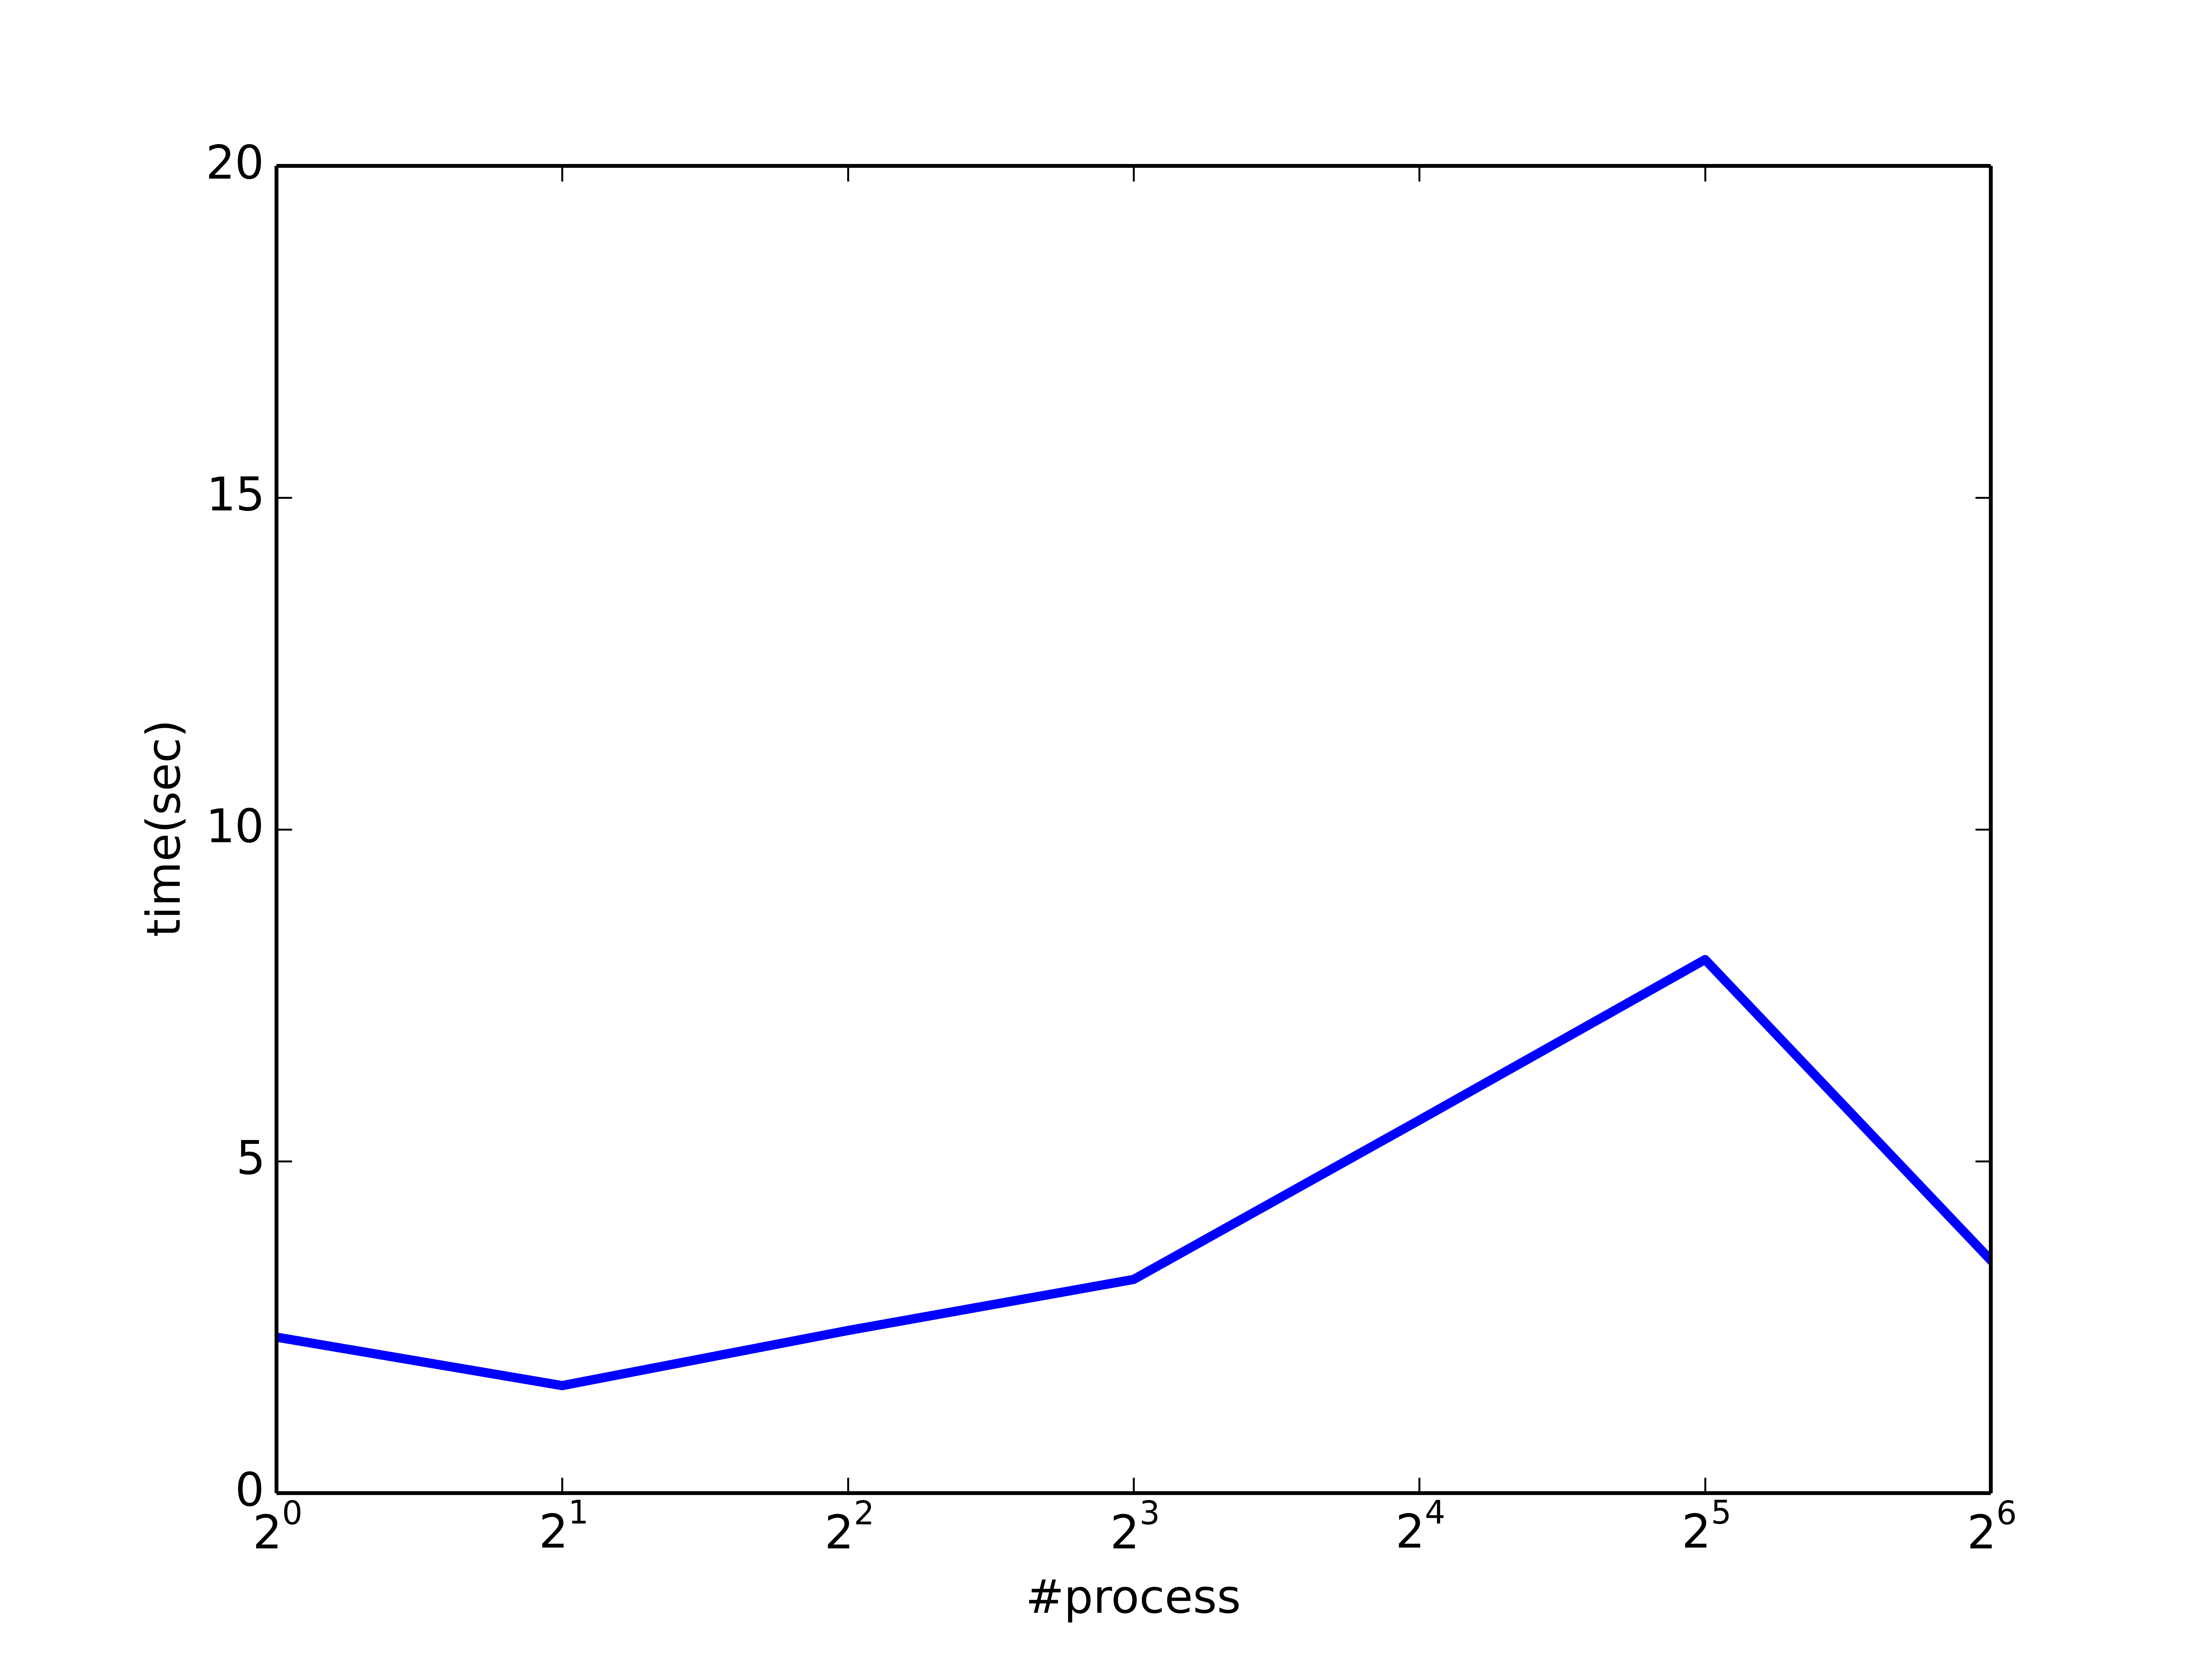
\includegraphics[width=0.5\textwidth]{ws.png}}\\
	\subfigure[strong scaling]{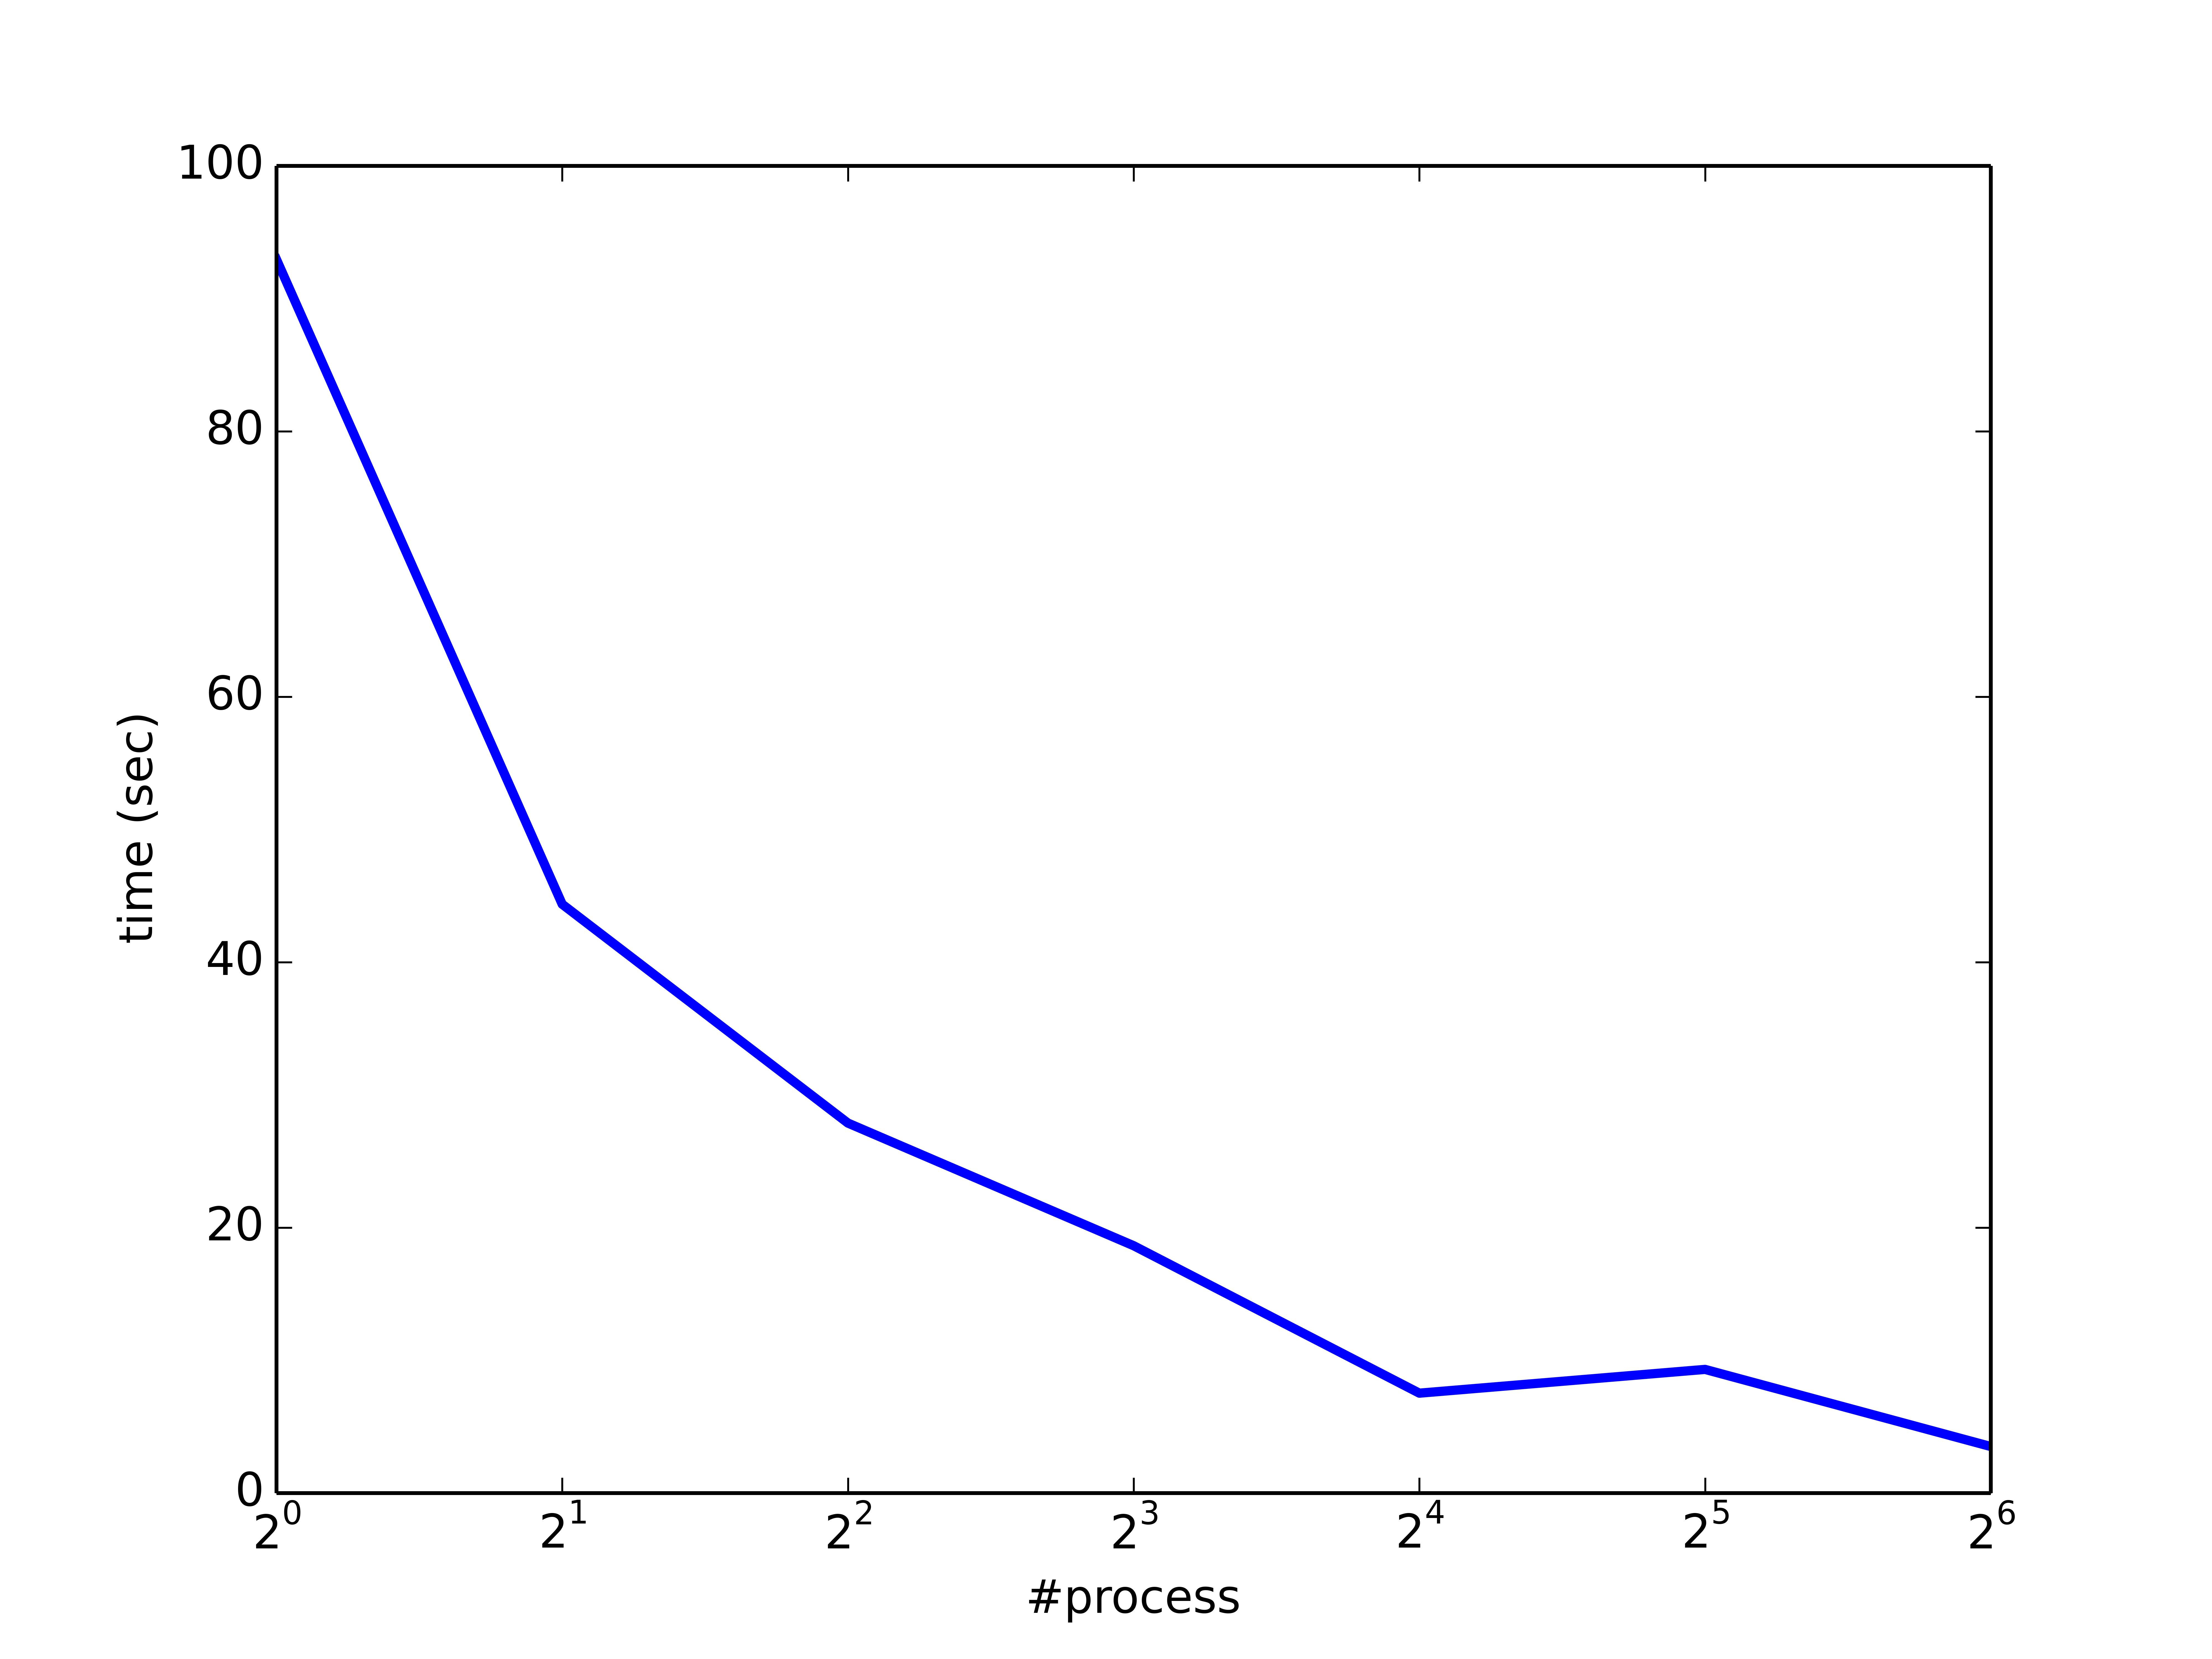
\includegraphics[width=0.5\textwidth]{ss1.png}}\\
	\subfigure[speedup with different algorithm parameters]{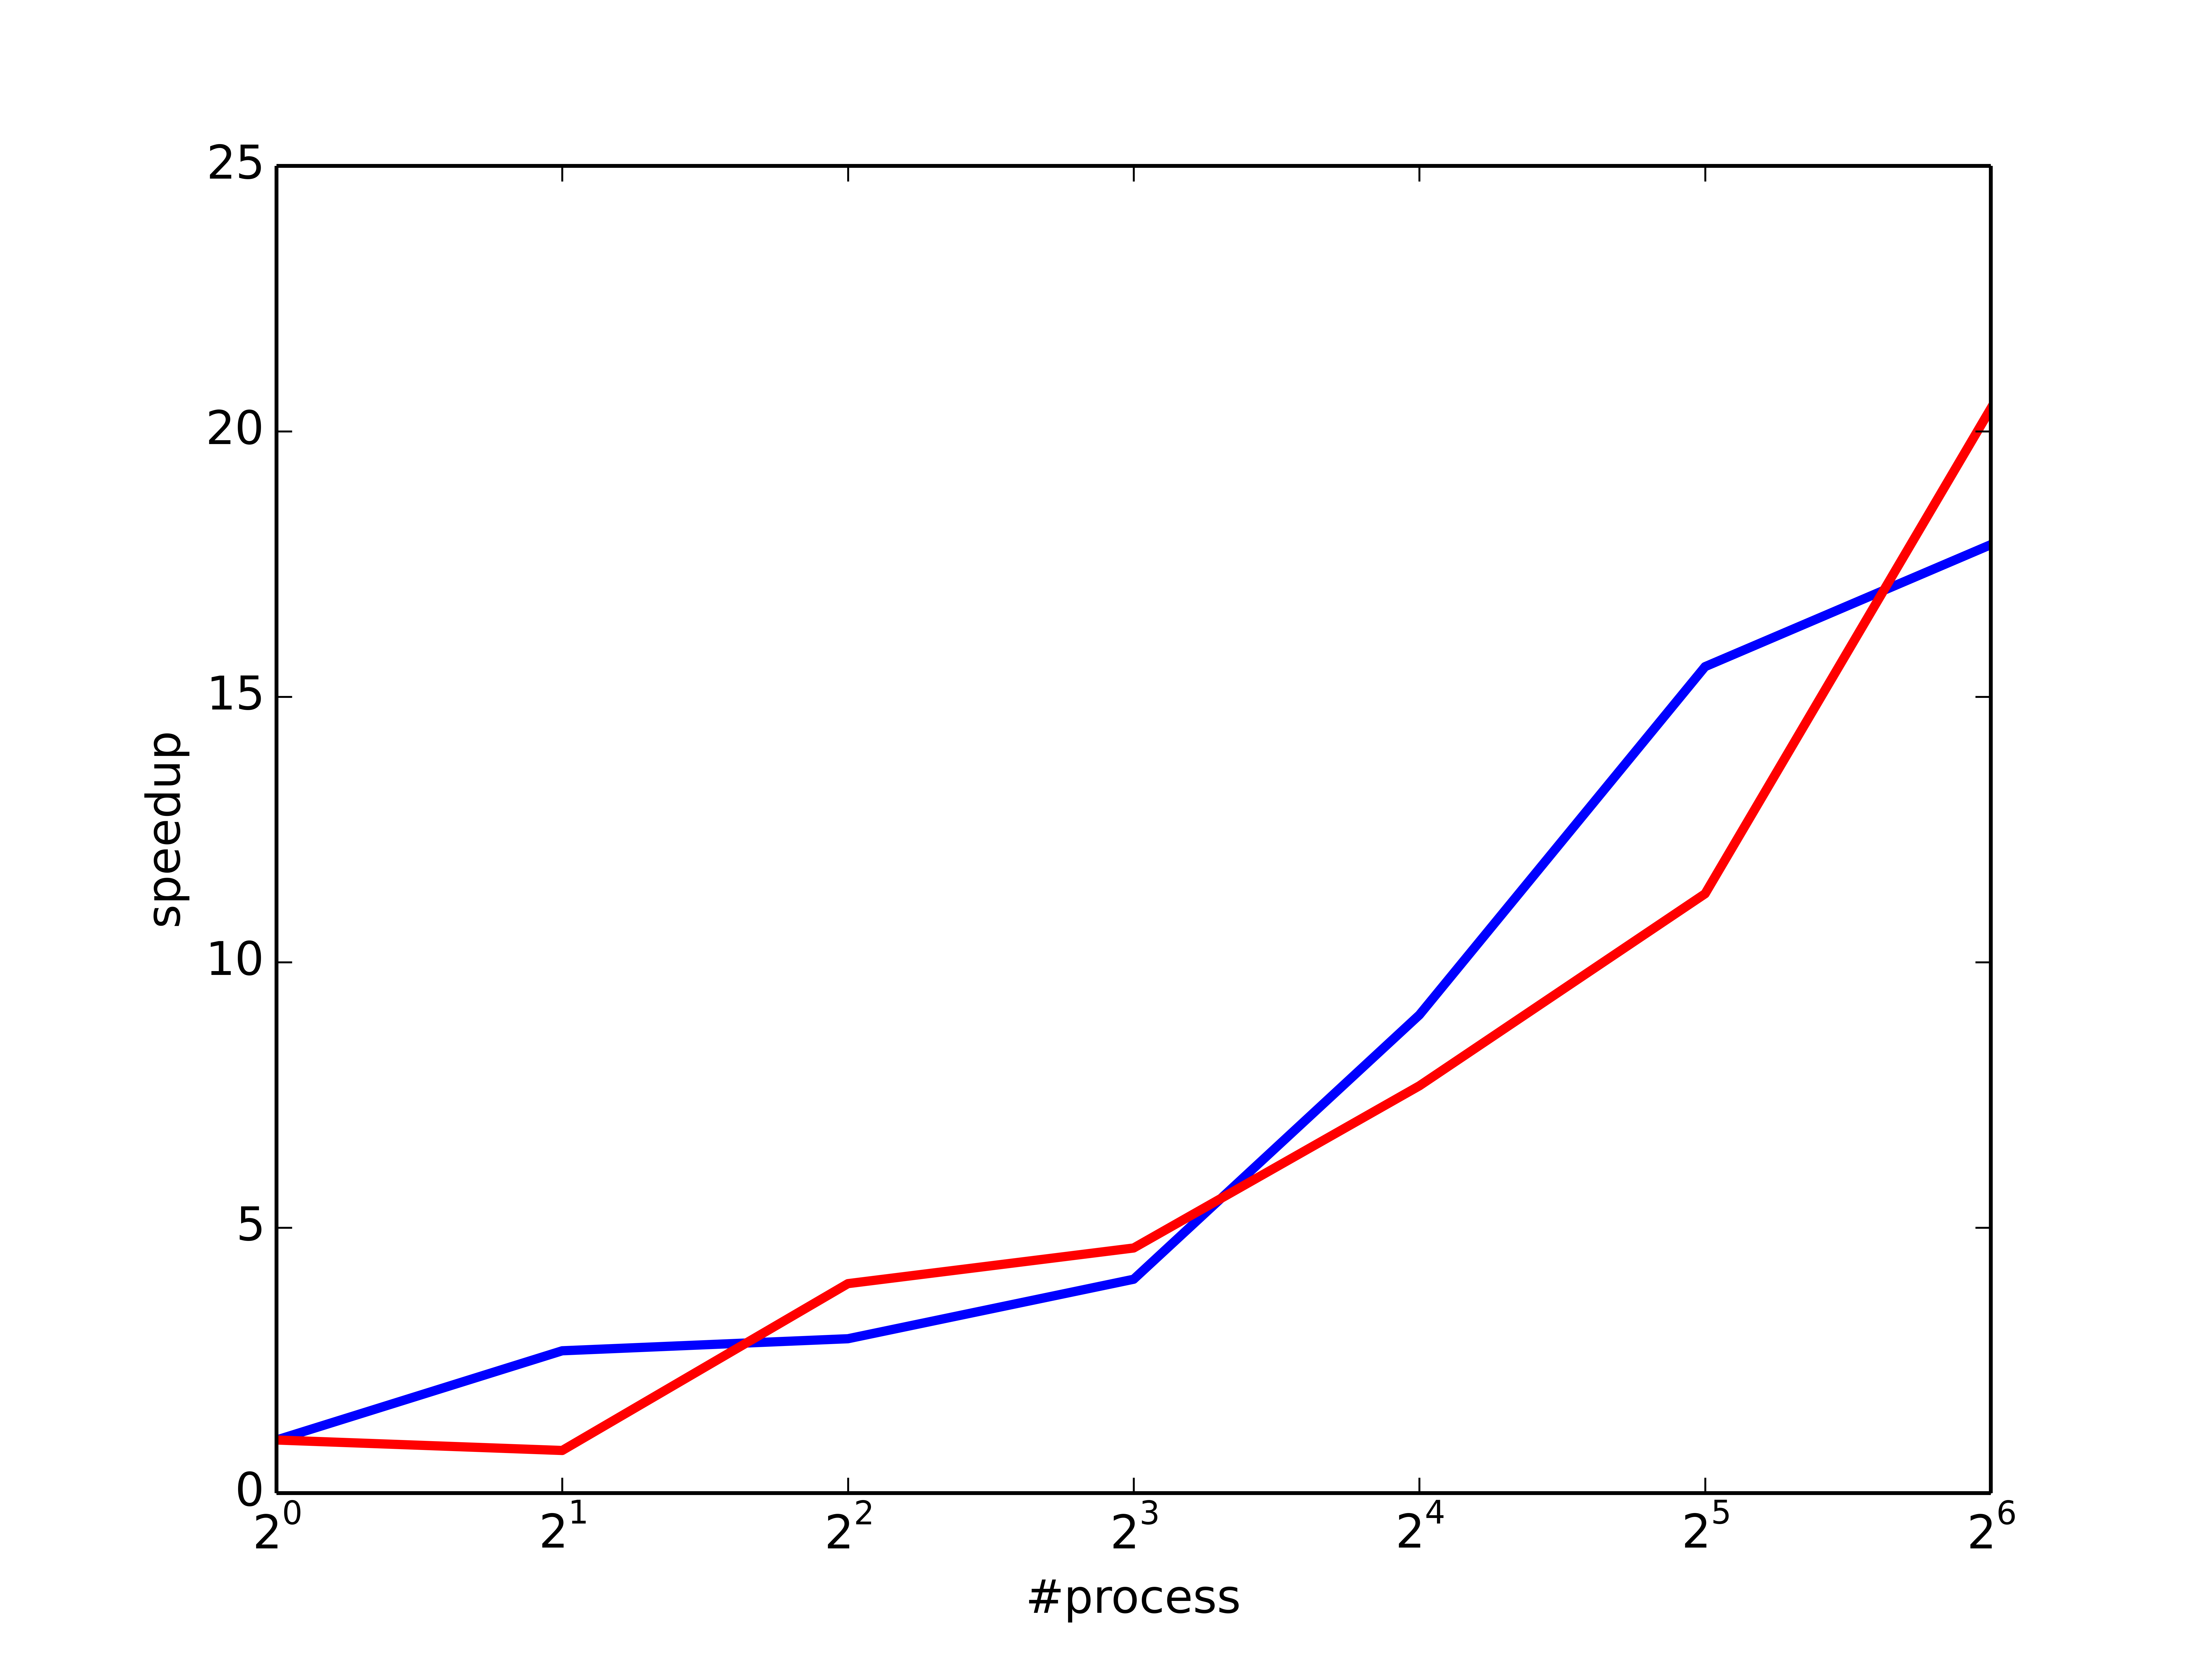
\includegraphics[width=0.5\textwidth]{su.png}}
	\caption{Scaling and speedup of parallel linear rankSVM with query-wise partition.}
	\end{figure}
\section{Conclusion}
From previous analysis and the experiment results, we can conclude that 
\begin{itemize}
\item Query-wise partition is more suitable when {$l \gg n$} ($q \ge M$), and feature-wise is more suitable when {$n \gg l$}. For $M \gg q$, the communication cost of QW increases while FW does not.
\item For large and dense data, the running time of the algorithm is dominated by computation cost and memory access, while for smaller and sparse data, it is dominated by communication cost.
\end{itemize}
\section{Future work}
There are something I would like to do in the future such as: doing more experiments on both large dense and sparse data; optimize the memory access; extend to kernel rankSVM \citep{TMK14a}.
\clearpage
\bibliography{my} 
\bibliographystyle{abbrvnat}
\end{document}